\section{Date: 2026-10-26}
\noindent \textbf{Series ID: NASDAQCX601020PI} 

\noindent This series is titled OMX Copenhagen Alternative Energy Price Index and has a frequency of Daily. The units are Index and the seasonal adjustment is Not Seasonally Adjusted.The observation start date is 2008-12-30 and the observation end date is 2026-10-23.The popularity of this series is 1. \\ 

\noindent \textbf{Series ID: POLRECDM} 

\noindent This series is titled OECD based Recession Indicators for Poland from the Peak through the Trough (DISCONTINUED) and has a frequency of Daily, 7-Day. The units are +1 or 0 and the seasonal adjustment is Not Seasonally Adjusted.The observation start date is 1995-02-01 and the observation end date is 2022-08-31.The popularity of this series is 1. \\ 

\subsection{Raw Regression}
\noindent Regresses the two series against each other directly. A significant result here can come just as easily from both series sharing a long-run trend as from any real relationship.

\begin{center}
\begin{tabular}{lclc}
\toprule
\textbf{Dep. Variable:}                & value\_fred\_POLRECDM & \textbf{  R-squared:         } &     0.057   \\
\textbf{Model:}                        &          OLS          & \textbf{  Adj. R-squared:    } &     0.057   \\
\textbf{Method:}                       &     Least Squares     & \textbf{  F-statistic:       } &     206.4   \\
\textbf{Date:}                         &    Mon, 26 Oct 2026   & \textbf{  Prob (F-statistic):} &  1.74e-45   \\
\textbf{Time:}                         &        17:43:09       & \textbf{  Log-Likelihood:    } &   -2167.1   \\
\textbf{No. Observations:}             &           3419        & \textbf{  AIC:               } &     4338.   \\
\textbf{Df Residuals:}                 &           3417        & \textbf{  BIC:               } &     4351.   \\
\textbf{Df Model:}                     &              1        & \textbf{                     } &             \\
\textbf{Covariance Type:}              &       nonrobust       & \textbf{                     } &             \\
\bottomrule
\end{tabular}
\begin{tabular}{lcccccc}
                                       & \textbf{coef} & \textbf{std err} & \textbf{t} & \textbf{P$> |$t$|$} & \textbf{[0.025} & \textbf{0.975]}  \\
\midrule
\textbf{const}                         &       0.4795  &        0.013     &    36.620  &         0.000        &        0.454    &        0.505     \\
\textbf{value\_fred\_NASDAQCX601020PI} &   -4.034e-05  &     2.81e-06     &   -14.366  &         0.000        &    -4.58e-05    &    -3.48e-05     \\
\bottomrule
\end{tabular}
\begin{tabular}{lclc}
\textbf{Omnibus:}       & 47995.954 & \textbf{  Durbin-Watson:     } &     0.009  \\
\textbf{Prob(Omnibus):} &    0.000  & \textbf{  Jarque-Bera (JB):  } &   514.195  \\
\textbf{Skew:}          &    0.676  & \textbf{  Prob(JB):          } & 2.21e-112  \\
\textbf{Kurtosis:}      &    1.665  & \textbf{  Cond. No.          } &  7.83e+03  \\
\bottomrule
\end{tabular}
%\caption{OLS Regression Results}
\end{center}

Notes: \newline
 [1] Standard Errors assume that the covariance matrix of the errors is correctly specified. \newline
 [2] The condition number is large, 7.83e+03. This might indicate that there are \newline
 strong multicollinearity or other numerical problems.

\begin{figure}
\centering
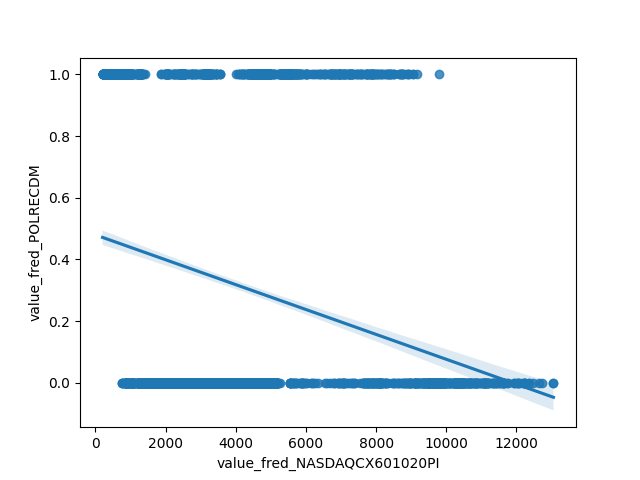
\includegraphics[scale = 0.9]{plots/plot_2026-10-26.png}
\caption{Raw Regression Plot for 2026-10-26}
\end{figure}
\newpage
\subsection{Detrended Regression}
\noindent Regresses the residuals of each series after removing its own linear time trend, so a shared trend can no longer drive the result on its own. A relationship that stays significant here is better evidence of a genuine link between the two series.

\begin{center}
\begin{tabular}{lclc}
\toprule
\textbf{Dep. Variable:}                           & value\_fred\_POLRECDM\_detrended & \textbf{  R-squared:         } &     0.071   \\
\textbf{Model:}                                   &               OLS                & \textbf{  Adj. R-squared:    } &     0.071   \\
\textbf{Method:}                                  &          Least Squares           & \textbf{  F-statistic:       } &     262.7   \\
\textbf{Date:}                                    &         Mon, 26 Oct 2026         & \textbf{  Prob (F-statistic):} &  5.73e-57   \\
\textbf{Time:}                                    &             17:43:09             & \textbf{  Log-Likelihood:    } &   -2123.7   \\
\textbf{No. Observations:}                        &                3419              & \textbf{  AIC:               } &     4251.   \\
\textbf{Df Residuals:}                            &                3417              & \textbf{  BIC:               } &     4264.   \\
\textbf{Df Model:}                                &                   1              & \textbf{                     } &             \\
\textbf{Covariance Type:}                         &            nonrobust             & \textbf{                     } &             \\
\bottomrule
\end{tabular}
\begin{tabular}{lcccccc}
                                                  & \textbf{coef} & \textbf{std err} & \textbf{t} & \textbf{P$> |$t$|$} & \textbf{[0.025} & \textbf{0.975]}  \\
\midrule
\textbf{const}                                    &   -2.884e-14  &        0.008     & -3.74e-12  &         1.000        &       -0.015    &        0.015     \\
\textbf{value\_fred\_NASDAQCX601020PI\_detrended} &   -7.539e-05  &     4.65e-06     &   -16.207  &         0.000        &    -8.45e-05    &    -6.63e-05     \\
\bottomrule
\end{tabular}
\begin{tabular}{lclc}
\textbf{Omnibus:}       & 113787.732 & \textbf{  Durbin-Watson:     } &     0.009  \\
\textbf{Prob(Omnibus):} &    0.000   & \textbf{  Jarque-Bera (JB):  } &   482.553  \\
\textbf{Skew:}          &    0.631   & \textbf{  Prob(JB):          } & 1.64e-105  \\
\textbf{Kurtosis:}      &    1.660   & \textbf{  Cond. No.          } &  1.66e+03  \\
\bottomrule
\end{tabular}
%\caption{OLS Regression Results}
\end{center}

Notes: \newline
 [1] Standard Errors assume that the covariance matrix of the errors is correctly specified. \newline
 [2] The condition number is large, 1.66e+03. This might indicate that there are \newline
 strong multicollinearity or other numerical problems.

\begin{figure}
\centering
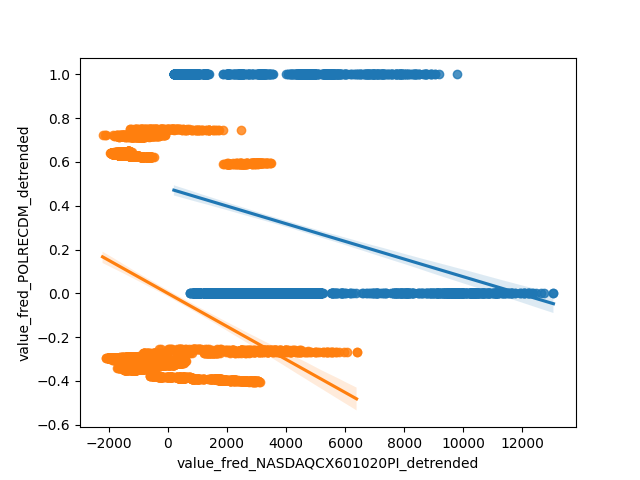
\includegraphics[scale = 0.9]{plots/plot_2026-10-26_detrended.png}
\caption{Detrended Regression Plot for 2026-10-26}
\end{figure}
\newpage
